\documentclass{article}
\usepackage{amsmath, amssymb, mdwlist, graphicx, hyperref}
\usepackage{listings,color}
\usepackage{wrapfig}
\usepackage[usenames,dvipsnames]{xcolor}
\definecolor{gray}{rgb}{0.97,0.97,0.97}
\lstset{%
language=Python,%
%backgroundcolor=\color{gray},
emph={putpixel},
emphstyle=\bf,
tabsize=4,
framesep=5pt,
mathescape=true,
xleftmargin=2cm,
xrightmargin=2cm,
frame=lines,
%basicstyle=\ttfamily,
%keywordstyle=\color{Blue},
%commentstyle=\color{OliveGreen},
%stringstyle=\color{MidnightBlue},
columns=flexible,
%showstringspaces=false
}

\newcommand{\mpar}[1]{\marginpar{\textit{#1}}}
\newcommand{\norm}[1]{\Vert #1 \Vert}
\DeclareMathOperator{\argmax}{argmax}
\DeclareMathOperator{\argmin}{argmin}
\newenvironment{solution}{\paragraph{Solution.}$\,$ }{\vskip 3mm\hrule}
\newenvironment{exercise}[2]{\begin{verse}\textbf{Exercise #1 (#2pt).} }{
\end{verse}\medskip}
\newcommand{\bbR}{\mathbb{R}}
\newcommand{\bw}{\mathbf{w}}
\newcommand{\bx}{\mathbf{x}}
\newcommand{\bd}{\mathbf{d}}
\newcommand{\bb}{\mathbf{b}}
\newcommand{\bs}{\mathbf{s}}
\newcommand{\by}{\mathbf{y}}
\newcommand{\bzero}{\mathbf{0}}
\newcommand{\bz}{\mathbf{z}}
\newcommand{\bSigma}{\mathbf{\Sigma}}
\newcommand{\bp}{\mathbf{p}}
\newcommand{\bm}{\mathbf{m}}
\newcommand{\bc}{\mathbf{c}}
\newcommand{\bM}{\mathbf{M}}
\newcommand{\bK}{\mathbf{K}}
\newcommand{\bD}{\mathbf{D}}
\newcommand{\bA}{\mathbf{A}}
\newcommand{\bX}{\mathbf{X}}
\newcommand{\bY}{\mathbf{Y}}
\newcommand{\bR}{\mathbf{R}}
\newcommand{\bI}{\mathbf{I}}
\newcommand{\bS}{\mathbf{S}}
\newcommand{\bT}{\mathbf{T}}
\newcommand{\balpha}{\boldsymbol{\alpha}}
\newcommand{\pt}[2]{\left(\begin{array}{c}#1\\#2\end{array}\right)}

\begin{document}
\title{MTAT.03.015 Computer Graphics (Fall 2013)\\
Exercise session VI: OpenGL. Blending. Auxiliary Buffers.}
\author{Konstantin Tretyakov, Ilya Kuzovkin}
\date{September 14, 2013}
\maketitle

In this practice we shall learn about blending and practice the use of the depth and stencil buffers. As usual, the base code is provided in the zip archive on the course website as well as in Github. Download, unpack and open it. You will need to submit your solution as a zipped archive file.

\section{Blending}
So far we have been assuming that during rasterization pixels are simply overwritten with appropriate color values. E.g. when you ask OpenGL to draw a blue triangle at a particular position, the pixels belonging to that triangle will all be set to blue. Quite often, however, you might want to \emph{blend} the new triangle with whatever is already drawn in the frame. 

To put it slightly more formally, suppose you are willing to draw with color $\bs = (r_s, g_s, b_s)$ onto a pixel that currently has color value $\bd = (r_d, g_d, b_d)$. \emph{Blending} means that instead of completely replacing the pixel's current value:
$$
\text{new\textunderscore pixel\textunderscore value} := \bs,
$$
the resulting value of the pixel will be a linear combination of its old and new colors:
$$
\text{new\textunderscore pixel\textunderscore value} := \lambda_1 \bs + \lambda_2 \bd\,.
$$

The coefficients $\lambda_1$ and $\lambda_2$ determine how much of an effect the original and the new color have on the result. The most common use of blending is imitating transparency via \emph{alpha-compositing}. For that, each color is augmented with the fourth component, commonly referred to as $\alpha$. An $\alpha = 1$ denotes full opacity, $\alpha = 0$ denotes full transparency, and values inbetween correspond to various levels of transparency. To implement alpha transparency using blending, we provide the value $\alpha_s$ with the color being drawn and compute the resulting pixel color as follows:
$$
\text{new\textunderscore pixel\textunderscore value} := \alpha_s \bs + (1-\alpha_s) \bd\,.
$$

Note that according to this rule, blending onto a pixel a new color with $\alpha_s = 1$ will completely overwrite the old value with the new one. Setting a color with $\alpha_s = 0$ will leave the old value intact. Using $\alpha_s = 0.5$ will result in an equal mixture of the old and new colors.

To use blending in OpenGL you have to do three things:
\begin{enumerate}
\item Enable it using \verb#glEnable(GL_BLEND);#.
\item Specify the $\lambda_1$ and $\lambda_2$ coefficients of the blending function using \\ \texttt{glBlendFunc(..)}. For example, to implement alpha-transparency you have to do:
\begin{verbatim}
   glBlendFunc(GL_SRC_ALPHA, GL_ONE_MINUS_SRC_ALPHA);
\end{verbatim}
Note that you have considerable freedom when configuring the blending coefficients (see the manual for \texttt{glBlendFunc}), which allows for some interesting uses. You can also change the addition to subtraction (see \texttt{glBlendEquation}).
\item Finally, you will need to specify the alpha component of all your colors using a four-component color function, e.g.:
\begin{verbatim}
   glColor4f(1.0, 0.0, 0.0, 0.5) // Semi-transparent red
\end{verbatim}
\end{enumerate}
In general, blending is slightly less efficient than writing pixels directly, so it is considered good practice to only enable blending for those primitives where it is required. However, rendering of anti-aliased (``smooth'') lines and polygons is only possible with alpha-transparency blending switched on.
\newpage
\begin{exercise}{1}{0.5}
Open the project \verb#1_Blending#. The first scene, described in the \verb#draw_triangles# function, renders three rotating triangles of different colors. First try making the triangles semi-transparent using alpha-compositing. See what happens if you set different alpha-values for different vertices of the blue triangle. Finally, to get points for the exercise configure blending to produce the picture below:
\begin{center}
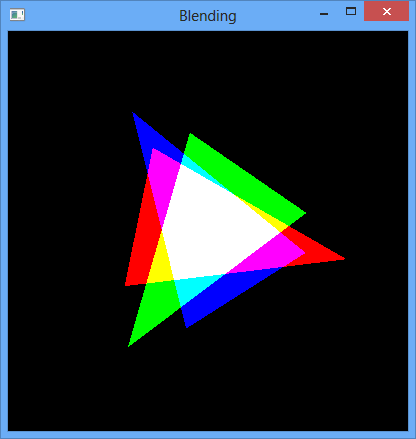
\includegraphics[width=0.5\textwidth]{blending.png}
\end{center}
\end{exercise}

\begin{exercise}{2}{0.5}
A common application for blending is to make effects such as \emph{motion blur}, \emph{soft shadows} or \emph{depth of field}. In the second scene of the project (function \verb#draw_motionblur#), implement the motion blur effect for a triangle. Currently the function renders 20 copies of the triangle, each shifted a bit to the right. To achieve a motion blur effect you have to configure blending so that each copy is multiplied by $1/20$, and all the copies are added together. This will effectively compute the \emph{average} of 20 different images. The result should look as follows:
\begin{center}
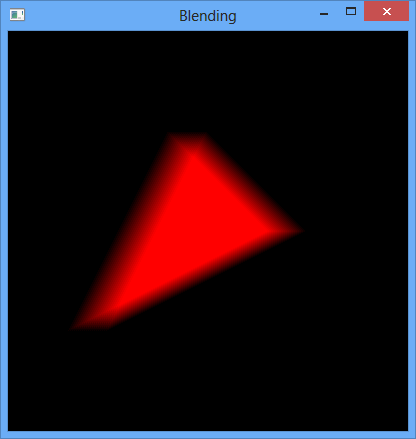
\includegraphics[width=0.5\textwidth]{motionblur.png}
\end{center}
\end{exercise}

\begin{exercise}{3*}{1}
Read about the method for implementing the Depth-of-Field effect\footnote{E.g. The Red Book, Chapter 10, \url{http://fly.cc.fer.hr/~unreal/theredbook/chapter10.html}}. Implement this effect on a simple scene with several objects at different distances from the camera. Use blending to implement it\footnote{Most probably the description you will find in the internet will refer to the use of \emph{accumulation buffer} for adding multiple frames. Accumulation buffer is, however, removed from the latest versions of OpenGL specification. Hence, to keep up with the times, I require you to use blending in this exercise as well.}. An example image you may strive for is the following:
\begin{center}
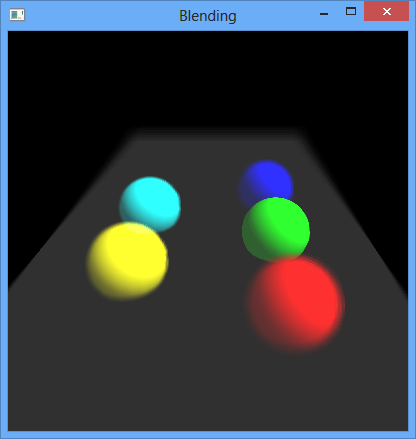
\includegraphics[width=0.5\textwidth]{dof.png}
\end{center}
\end{exercise}

Note that blending is a general concept, not specific to OpenGL. For example, the same notions apply to Allegro (see \verb#al_set_blender#).

\section{Depth Buffer}
In the lecture we learned about the \emph{Z-buffer} (a.k.a \emph{depth buffer}) algorithm. The simple take-away message there was that you should always have it enabled when working with 3D graphics. Let us now practice the use of the depth buffer on an (admittedly somewhat artificial) example\footnote{Think how you could achieve the same effect without resorting to depth buffer manipulations}.

\begin{exercise}{4}{0.5}
Open the project \verb#2_DepthBuffer#. It contains a rendering of a model, that should be familiar to you from practice session 4. Suppose we would like to render only the part of the model, that lies closer to the camera than distance 6 (which is the distance to the center of the model). Image below illustrates the desired effect.
\begin{center}
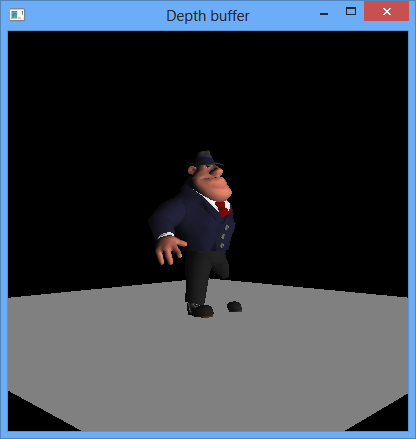
\includegraphics[width=0.5\textwidth]{halfmodel.png}
\end{center}

To achieve this effect using the depth buffer do the following:
\begin{enumerate}
\item Draw the floor rectangle (\verb#draw_floor#) as usual.
\item Switch off drawing to the screen using \texttt{glColorMask}. Now you will only render to the depth buffer.
\item Draw a large rectangle (e.g. $100\times 100$) at distance $6$ from the viewer. (Recall that in the camera frame the $z$ axis points straight out of the screen).
\item Switch drawing to the screen back on and render the model as usual.
\end{enumerate}

Implement this in \verb#2_DepthBuffer#.
\end{exercise}

\section{Stencil Buffer}
Another useful auxiliary buffer is the \emph{stencil buffer}. Like the depth buffer, it keeps a separate value for each pixel, however the values are integers. You can specify an operation used to update the stencil buffer using \texttt{glStencilOp}. 

For example, \verb#glStencilOp(GL_INCR, GL_INCR, GL_INCR)# specifies that the value in the stencil buffer has to be increased each time a pixel could be drawn to it. Hence, if you start with a zeroed stencil buffer and render the whole scene, each value in the stencil buffer will count how many triangles were rendered at that pixel.

In addition to the buffer update rule, you may specify a \emph{stencil test}, which lets you decide on a pixel-per-pixel basis, which pixels should be drawn, depending on their stencil values. You enable the stencil test using \\ \verb#glEnable(GL_STENCIL_TEST)# and specify the type of test using \verb#glStencilFunc#.

Stencil buffer allows to implement numerous interesting effects, such as shadows, reflections, contours or object intersections. Here we shall use it to implement a simple reflection.

\begin{exercise}{5}{1}
Open project \verb#3_StencilBuffer# and modify it as follows:
\begin{enumerate}
\item Modify \texttt{glutInitDisplayMode} to allocate memory for the stencil buffer. Enable the stencil test.
\item Modify \texttt{display} function to implement the following algorithm:
\begin{enumerate}
\item Clear the frame, depth and stencil buffers
\item Render the floor \emph{only} to the stencil buffer (disable writing to depth or color buffers temporarily), setting stencil buffer values to $1$ for all pixels of the floor.
\item Set the stencil test to pass only for pixels that have stencil buffer value of $1$. Render the figure of a man, mirrored about the $y=0$ plane. Due to stenciling, only ``floor'' pixels will be affected.
\item Set the stencil test to always pass. Render the floor, using alpha-transparency with a coefficient of $0.8$ for the floor.
\item Finally, render the man standing on the floor as normal.
\end{enumerate}
\end{enumerate}
The result should look as the image below.
\begin{center}
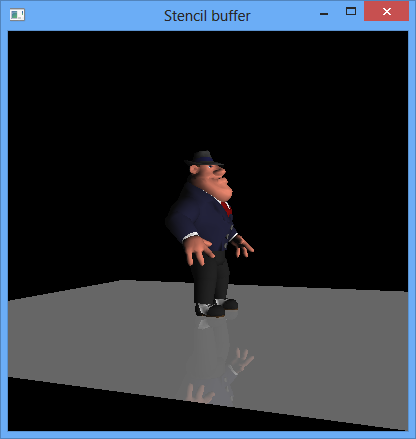
\includegraphics[width=0.6\textwidth]{stencil.png}
\end{center}

\end{exercise}

\end{document}
